\documentclass{beamer}

%%% Проверка используемого TeX-движка %%%
\usepackage{ifxetex}

%%% Кодирование и шрифты %%%
\ifxetex
\usepackage{polyglossia}                         % Поддержка многоязычности
\usepackage{fontspec}                            % TrueType-шрифты
\else
\usepackage{cmap}                                % Улучшенный поиск русских слов в полученном pdf-файле
\usepackage[T2A]{fontenc}                        % Поддержка русских букв
\usepackage[utf8]{inputenc}                      % Кодировка utf8
\usepackage[english, russian]{babel}             % Языки: русский, английский
\fi
\usepackage{listings}

%%% Математические пакеты %%%
\usepackage{amsthm,amsfonts,amsmath,amssymb,amscd} % Математические дополнения от AMS

%%% Оформление абзацев %%%
\usepackage{indentfirst}                           % Красная строка

%%% Оформление кода %%%
\lstset{
    language=Java,
    basicstyle=\tiny\sffamily,
    numbers=left,
    numberstyle=\tiny,
    tabsize=4,
    columns=fixed,
    showstringspaces=false,
    showtabs=false,
    keepspaces,
    commentstyle=\color{red},
    keywordstyle=\color{blue}
}

% Стиль презентации
\usetheme{Warsaw}

\newcommand{\br}{\pause \linebreak \linebreak}
\newcommand{\nl}{\pause \linebreak}

\begin{document}
\title{Сортировка расчёской}
\author{Лев Захаров}
\institute{Высшая школа ИТИС КФУ}
\date{Казань, 2015}
% Создание заглавной страницы
\frame{\titlepage}
% Автоматическая генерация содержания
\frame{\frametitle{Содержание}\tableofcontents}

\section{Вступление}
\begin{frame}
    \frametitle{Вступление}
    	\alert{Сортировка расческой} - модификация сортировки пузырьком, позволяющая ощутимо ускорить время работы алгоритма.
\end{frame}

\section{Алгоритм}
\begin{frame}
    \frametitle{Во всем виноваты черепашки}
	 \center\includegraphics[width=3.3in]{turtle}
\end{frame}

\begin{frame}
   	\alert{Черепаха} $-$ элемент с относительно маленьким значением, находящийся в конце списка.
        \nl
        \alert{Кролик} $-$ элемент с относительно большим значением, находящийся в начале списка.
        \br
        В процессе сортировки черепашки сдвигаются только на одну позицию за один проход. С другой стороны \textit{кролики} двигаются достаточно быстро.
\end{frame}

\begin{frame}
    \frametitle{Сортировка расческой}
    Основная идея сортировки расческой заключается в том, чтобы первоначально выбирать расстояние между сравниваимыми элементами больше еденицы.
    \br
    Для первого прохода шаг равен частному от деления размера массива на \alert{фактор уменьшения}.
    \nl
    На каждом последующем шаге расстояние между сравниваемыми элементами делится на \alert{фактор уменьшения}.
    \br
    Так продолжается до тех пор, пока разность индексов сравниваемых элементов не достигнет единицы.
    Дальше массив досортировывается пузырьком.
\end{frame}

\begin{frame}
    \frametitle{Фактор уменьшения}
    Опытным и теоретическим путем было установлено оптимальное значение \alert{фактора уменьшения}:
    \begin{center}
        \Large $\frac{1}{1 - \frac1{e^{\varphi}}} \thickapprox 1.247330950103979$
    \end{center}
    , где $\varphi$ есть золотое сечение, т.е. $\varphi = \frac{1 + \sqrt{5}}2$.
\end{frame}

\section{Реализация}
\begin{frame}
    \frametitle{Реализация}
    \lstinputlisting{CombSort.java}
\end{frame}

\section{Оценка сложности}
\begin{frame}
    \frametitle{Зависимости времени работы от размера массива}
    \begin{figure}
        \center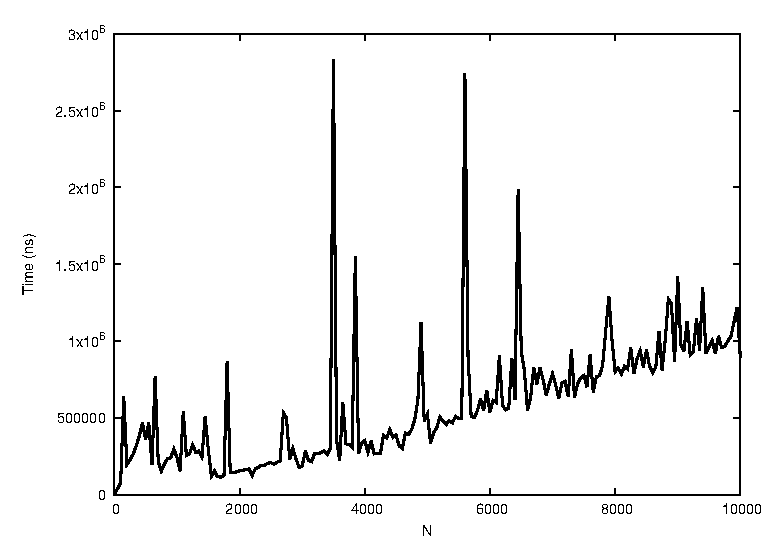
\includegraphics[width=3.3in]{g1}
    \end{figure}
\end{frame}
\begin{frame}
    \frametitle{Зависимость итераций от размера массива}
    \begin{figure}
        \center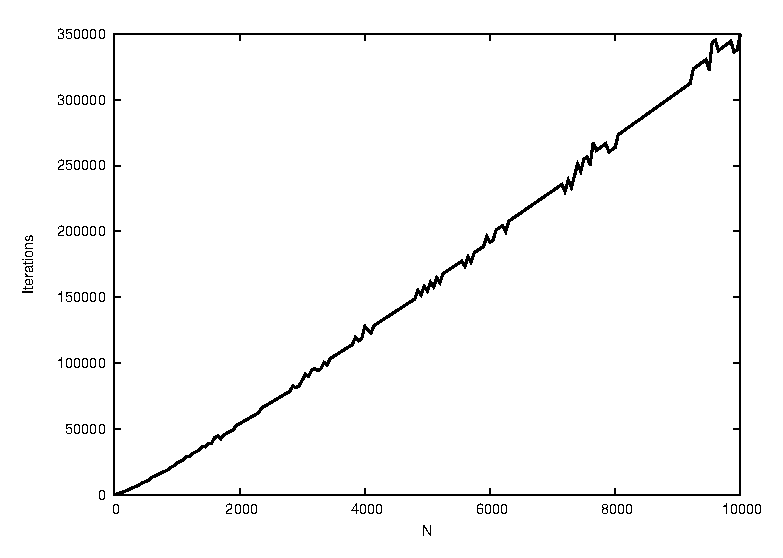
\includegraphics[width=3.3in]{g2}
    \end{figure}
\end{frame}
\begin{frame}
    \frametitle{Вычислительная сложность алгоритма}
    Вычислительная сложность сортировки расческой в среднем равна $O(n\log{n})$, и $O(n^2)$ в худшем случае.
    \br
    Сортировка расческой конкурирует с алгоритмами, подобными быстрой сортировке.
\end{frame}

\section{Вывод}
\begin{frame}
    \frametitle{Вывод}
    \textcolor{blue}{Плюсы:}
    \begin{itemize}
    	\item{Алгоритм сортировки является простым для понимания и легкореализуемым.}
	\item{В среднем работает значительно быстрее сортировки пузырьком и на некоторых входных данных опережает по сложности быстрые сортировки.}
    \end{itemize}
    \textcolor{red}{Минусы:}
    \begin{itemize}
    	\item{Алгоритм неустойчив.}
	\item{На некоторых данных деградирует до квадратичной сложности.}
    \end{itemize}

\end{frame}

\section{Список литературы}
\begin{frame}
    \frametitle{Список литературы}
    \begin{thebibliography}{3}
        \setbeamertemplate{bibliography item}[online]
        \bibitem{4} {Пузырьковая сортировка и все-все-все} {\tiny{http://habrahabr.ru/post/204600/}}
        \setbeamertemplate{bibliography item}[article]
        \bibitem{C} {\bf A Fast Easy Sort},
            Byte Magazine, April 1991
    \end{thebibliography}
\end{frame}

\end{document}